\section{Ejercicio 3}

Definimos el peso de un nodo como la suma de los pesos de las aristas que inciden sobre él. La idea de la heurística golosa constructiva es entonces ``aislar'' a los nodos más pesados, bajo la premisa de que éstos son los más problemáticos y deben ser los primeros en procesarse.

Lo que se hace en un principio es agarrar el nodo más pesado, y agregarlo a un conjunto. Después, se busca el nodo más pesado de los no asignados, y se pone en el mejor conjunto disponible. El criterio para elegir a un conjunto es el peso del nodo en ese conjunto. Y así siguiendo hasta que no haya mas nodos. El pseudocódigo es:
\begin{algorithm}[H]
\begin{algorithmic}[1]
\caption{HeuristicaGolosaConstructiva(Grafo G, nat k)}
\STATE Vector$<$Conjunto$<$Nat$>>$ conjuntos(k, vacío)
\IF {k $\geq$ n}
    \STATE CompletarConSolucionTrivial(conjuntos, n) \textcolor{CadetBlue}{// conjuntos$[$i$]$ $=$ i $\forall$ nodo i $\in$ G}
\ELSE
    \STATE Vector$<$Nat$>$ nodosOrdenados $\leftarrow$ OrdenarNodosPorPesoMayorAMenor(G)
    \FOR {\textbf{each} vértice de nodosOrdenados}
        \STATE pesoMinimo $\leftarrow$ $+ \infty$
        \STATE mejorConjunto $\leftarrow$ 0
        \FOR {i = 0 \TO k - 1}
            \STATE pesoEnConjunto $\leftarrow$ PesoVerticeEnConjunto(vértice, conjuntos$[$i$]$)
            \IF { pesoEnConjunto $<$ pesoMinimo }
                \STATE pesoMinimo $\leftarrow$ pesoEnConjunto
                \STATE mejorConjunto $\leftarrow$ i
            \ENDIF
        \ENDFOR
        \STATE conjuntos$[$mejorConjunto$]$.insertar(vértice)
    \ENDFOR
\ENDIF
\RETURN conjuntos
\end{algorithmic}
\end{algorithm}

Por ejemplo, en el grafo de la Figura \ref{fig:ej3_ejemplo} (para cada nodo se aclara entre paréntesis su peso) para k = 2 --es decir, la solución son los conjuntos $\left\{S_1, S_2\right\}$ siendo ambos vacíos al inicio--. El algoritmo hace lo siguiente: Supongamos que el orden de los nodos por peso dió $[F, C, A, E, B, D]$.Toma el nodo $F$ porque es el más pesado (tiene peso 11) y lo agrega en $S_1$. Después toma $C$ que tiene peso 9, y lo pone en $S_2$, que sigue vacío (el peso de $C$ en $S_1 = \{$F$\}$ es 3 porque $C$ y $F$ son adyacentes con una arista de peso 3). Hasta ahora tenemos la partición $\left\{ \left\{F\right\}, \left\{C\right\} \right\}$. Los nodos $A$ y $E$ tienen ambos peso 8, por el orden ya predefinido toma el vértice $A$ y lo pone en el mejor conjunto, que es $S_2$ --ahí tiene peso 2-- mientras que en $S_1$ tiene peso 3. Tenemos entonces $\{ \{F\}, \{C, A\} \}$. El nodo $E$ tiene peso 5 en $S_1$ por su arista con $F$ y peso 2 en $S_2$ a pesar de ser adyacentes a ambos nodos del conjunto, por lo tanto se pone ahí. Siguiendo el mismo razonamiento, el algoritmo pone a $B$ en $S_1$ y luego a $D$ en $S_1$. Finalmente, queda lo que muestra la Figura \ref{fig:ej3_ejemplo_solucion}. Notar como los nodos más pesados tienden a estar más aislados, en particular el nodo $F$ lo está completamente. Notar también que las aristas más pesadas (de peso $\geq$ 3) no forman parte de ningún conjunto de la partición calculada por la heurística.

\begin{figure}[H]
	\begin{minipage}[t]{0.5\linewidth}
		\centering
		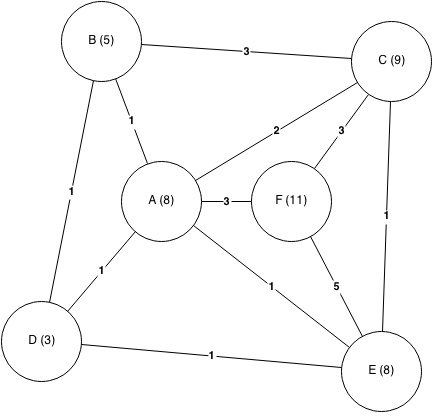
\includegraphics[width=\textwidth]{ejercicio-3-ejemplo-entrada.png}
		\caption{Grafo de entrada}
		\label{fig:ej3_ejemplo}
	\end{minipage}
	\begin{minipage}[t]{0.5\linewidth}
		\centering
		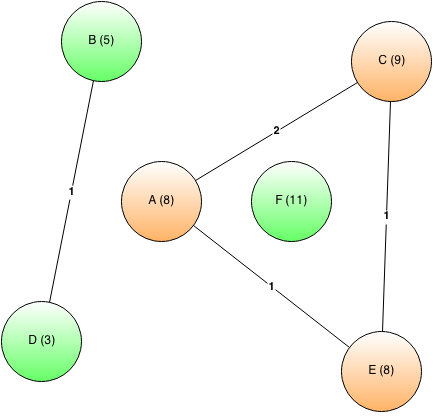
\includegraphics[width=\textwidth]{ejercicio-3-ejemplo-salida.png}
		\caption{La solución dada por la heurística, diferenciada con colores}
		\label{fig:ej3_ejemplo_solucion}
	\end{minipage}
\end{figure}

El problema de la heurística es que solamente compara el peso de un nodo con los conjuntos, sin tener en cuenta el resto de los nodos aún no asignados. Esto puede dar soluciones tan alejadas de la óptima como queramos. A saber:

Sea G un grafo cuyas aristas tienen peso 1, y k el parámetro de k-PMP. Es decir, el grado de un vértice es igual a su peso. G tiene dos tipos diferentes de nodos:
\begin{itemize}
    \item Los nodos $P_1, ..., P_k$ forman un subgrafo completo. Entonces, $d(P_i) = k-1$ en ese subgrafo.
    \item Los nodos $L_1, ..., L_N$ verifican que cada $L_i$ es solamente adyacente a todos los nodos $P_i$. Es decir, $d(L_i) = k$ para todo $i = 1, ..., N$.
\end{itemize}
Por lo anterior, los nodos $P_i$ tienen grado $N+k-1$. Estos nodos van a ser más pesados que los $L_i$ cuando $N > 1$, pues 
\begin{align*}
N+k-1 > k \Longleftrightarrow N > 1
\end{align*}
Supongamos entonces que hay más de un nodo de tipo $L$. Notemos además que el conjunto $\{L_1, ..., L_N\}$ tiene peso cero, ya que ningún par de nodos es adyacente entre sí.
Como el algoritmo ordena por peso de mayor a menor, el orden será del tipo 
\begin{align*}
[P_{i_1},...,P_{i_k},L_{j_1},...,L_{j_N}]
\end{align*}
Entonces, si N $>$ 1, el algoritmo va a elegir un nodo $P$ hasta que se terminen. A $P_{i_1}$ lo va a poner en $S_1$. A $P_{i_2}$ no lo puede poner en $S_1$ porque tiene peso 1 ahí (es adyacente a $P_{i_1}$, por lo tanto lo pone en $S_2$ que está vacío. A $P_{i_3}$ no puede ponerlo ni en $S_1$ ni en $S_2$ por la misma razón, entonces lo pone $S_3$. Así, una vez terminados todos los nodos $P$, la partición es
\begin{align*}
\{\{P_{i_1}\},\{P_{i_2}\},...,\{P_{i_k}\}\}
\end{align*}
Queda insertar los N nodos restantes, que son los $L_{j_1},...,L_{j_N}$. Pero para cualquiera de estos nodos, su peso en $S_x$ es 1 porque es adyacente a $P_{i_x}$. Como el algoritmo elige al primer conjunto y después chequea si eligiendo los demás mejora, y no lo hace en este caso, todos van a ir a $S_1$. Por lo tanto, la solución dada por el algoritmo será
\begin{align*}
\{ \{P_{i_1}, L_1, L_2, ..., L_N\}, \{P_{i_2}\}, ..., \{P_{i_k}\} \}
\end{align*}
El peso total de esta solución es N.
Pero si la solución fuera
\begin{align*}
\{ \{L_1, L_2, ..., L_N\}, \{P_{i_1}, P_{i_2}\}, ..., \{P_{i_k}\} \}
\end{align*}
el peso total sería 1. Es decir, la solución dada por la heurística golosa puede ser tan mala como queramos. Veamos gráficamente para k = 3 la diferencia:
\begin{figure}[H]
	\begin{minipage}[t]{\linewidth}
		\centering
		\frame{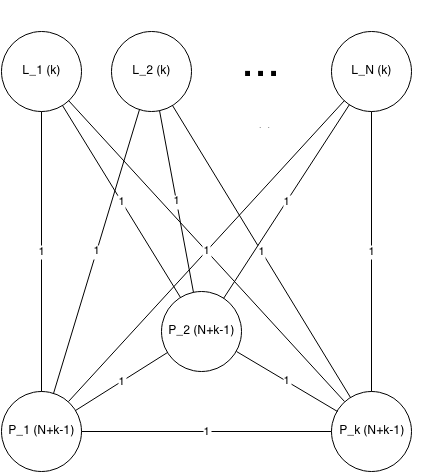
\includegraphics[width=0.5\textwidth]{ejercicio-3-rotura-heuristica.png}}
		\caption{Grafo de entrada}
		\label{fig:ej3_rotura_entrada}
	\end{minipage}
\end{figure}
\begin{figure}[H]
	\begin{minipage}[t]{0.5\linewidth}
		\centering
		\frame{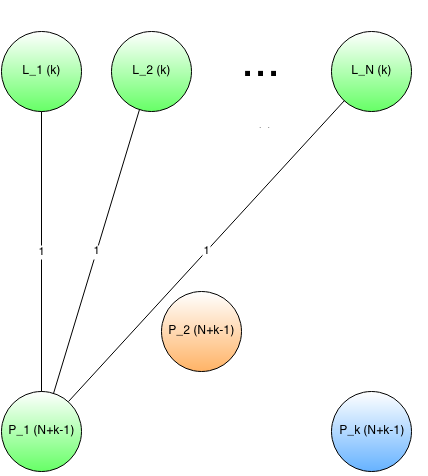
\includegraphics[width=\textwidth]{ejercicio-3-rotura-heuristica-solucion-golosa.png}}
		\caption{Solución golosa, con peso N.}
		\label{fig:ej3_rotura_golosa}
	\end{minipage}
	\begin{minipage}[t]{0.5\linewidth}
		\centering
		\frame{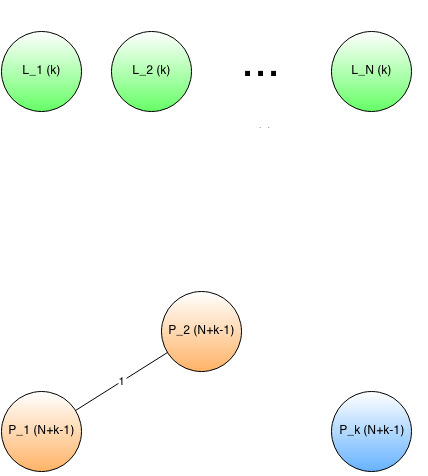
\includegraphics[width=\textwidth]{ejercicio-3-rotura-heuristica-solucion-optima.png}}
		\caption{Una solución óptima, con peso 1.}
		\label{fig:ej3_rotura_optima}
	\end{minipage}
\end{figure}

\subsection{Análisis de complejidad temporal}

Sea $n$ la cantidad de vértices del grafo de entrada, y $k$ el parámetro de k-PMP. Vamos a usar el pseudocódigo ya introducido para el cálculo de complejidad:
\begin{enumerate}
    \item En la primera línea se crean $k$ conjuntos vacíos. Esto cuesta $O(k)$. Llamaremos $C_i$ al i-ésimo conjunto. El caso poco interesante es que sea $k \geq n$. Se toma como solución (que de hecho es óptima) la partición 
    \begin{align*}
    \{\{v_1\}, \{v_2\}, ..., \{v_n\}, \{\}, ..., \{\}\}
    \end{align*}
    que tiene peso total cero. Insertar los nodos cuesta $O(n)$, y ahí terminaría el algoritmo, cuya complejidad temporal total sería $O(k)$. Pasemos al caso relevante, que es $k < n$.
    \item Se crea un vector de tamaño $n$, con los vértices ordenados por peso en el grafo, de mayor a menor. Preguntarle a un vértice su peso en el grafo cuesta $O(n)$ porque representamos al grafo con una matriz de adyacencia, entonces en total es $O(n^2)$ saber el peso de todos los nodos. Finalmente, ordenar las tuplas $<nodo,peso(nodo)>$ cuesta $O(n \log n)$. Por lo tanto, todo esto cuesta $O(n^2)$. Al nodo i-ésimo de este nuevo ordenamiento lo llamaremos $u_i$.
    \item Ahora para cada $u_i$ se hace lo siguiente:
        \begin{enumerate}
            \item Inicializar las variables $pesoMinimo$ y $mejorConjunto$ cuesta $O(1)$.
            \item Para cada conjunto $C_i$ de la partición, se calcula el peso de $u_i$ en él y se chequea si es mejor para cambiar el $mejorConjunto$. El peso en un $C_i$ se calcula simplemente sumando los pesos de la aristas adyacentes entre $u_i$ y los vértices del conjunto, lo cual lleva $O(|C_i|)$. Sabemos que
            \begin{align*}
                \sum\limits_{\substack{i = 1}}^k |C_i| &= i - 1
            \end{align*}
            (pues sólo se asignaron $i - 1$ nodos en la iteración i-ésima). Por otro lado, estamos iterando sobre $k$ conjuntos, entonces el costo de este paso es $O(k) + O(i - 1)$.
            \item Insertar el nodo en $mejorConjunto$ cuesta $O(\log |mejorConjunto|)$ que podemos acotar por $O(\log (i - 1))$.
        \end{enumerate}
        En total, todo este paso cuesta
        \begin{align*}
                \sum\limits_{\substack{i = 1}}^n (O(k) + O(i-1) + O(\log (i - 1))) &= O(nk) + O(n^2) + O(\log n!)
        \end{align*}
        Por la aproximación de Stirling del factorial ($\log n! = n \log(n) - n + O(\log n)$), tenemos que $O(\log n!) = O(n \log n)$, entonces la complejidad total de este paso es $O(nk) + O(n^2)$.
\end{enumerate}
Tenemos entonces que la complejidad temporal de la heurística golosa es
\begin{align*}
    T(n,k) &= O(k) + O(n^2) + O(nk) + O(n^2) \\
    T(n,k) &= O(nk) + O(n^2)
\end{align*}
Como tomar valores $k \geq n$ no tiene sentido, ya que una solución óptima es trivial, entonces siendo $k < n$ vale que $O(nk) = O(n^2)$. Por lo tanto, la complejidad temporal de peor caso de la heurística para un tamaño de entrada de $n$ vértices es
\begin{align*}
    T(n) &= O(n^2)
\end{align*}

\subsection{Test de complejidad}

Construimos 100 instancias aleatorias de grafos de $n$ vértices, para cada $n = {1, ... , 100}$. Para cada instancia, se calculó el tiempo de ejecución de la heurística con parámetro $k = {10, 20, ..., 100}$ cinco veces (tomando el mínimo), para luego calcular el promedio para cada $n$ separando por $k$. Así, para cada $n$ tenemos el tiempo de ejecución promedio de cada $k$. Como esperamos que la complejidad temporal sea $O(n^2)$ se dividió la muestra por $n$, esperando ver una recta, que es lo que efectivamente ocurre. Veamos el gráfico de los resultados del test:

\begin{figure}[H]
    \begin{minipage}[t]{\linewidth}
		\centering
		\frame{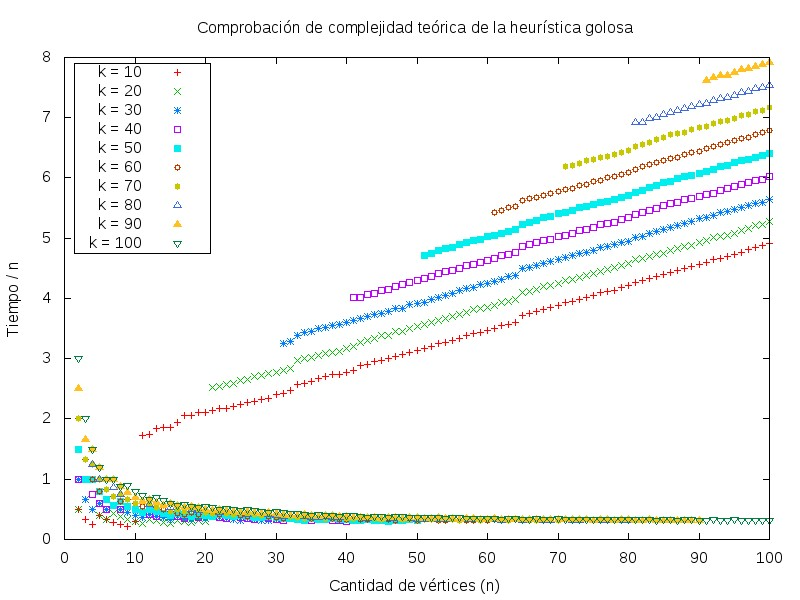
\includegraphics[width=\textwidth]{ejercicio-3-complejidad-dividida-n.jpg}}
		\label{fig:ejercicio_3_complejidad_dividida_n}
    \end{minipage}
\end{figure}

Podemos observar que para cada $n \leq k$, el tiempo dividido por $n$ es una constante, lo cual tiene sentido porque habíamos acotado por $O(k)$ construir la solución trivial, y $O(n) \subseteq O(k)$ porque $n \leq k$. Recién a partir de $n = k+1$ el tiempo dividido $n$ se vuelve apreciable, y como esperábamos es una recta, lo que indica que es $O(n^2)$ como era nuestra hipótesis.

